\documentclass{article}
\usepackage[utf8]{inputenc}
\usepackage{amsmath}
\usepackage{amsfonts}
\usepackage{tikz}
\usepackage{tkz-euclide}
\usepackage{graphicx}
\usepackage{nopageno}
\graphicspath{ {./images/} }

\begin{document}

\begin{center}
        \section*{Maths Problems Set 4 (24 March 2020)}
\end{center}

\begin{enumerate}
    \item
    5 points are placed in a $1\times1$ square. Show that no matter where the points are placed there will always be a pair of points with a distance of less than or equal to $\frac{1}{\sqrt{2}}$ between them.

    
    \item
    A positive integer ends in the digit 4 and has the property that it becomes four times as large when the 4 is moved from the end and placed at the front. What is the smallest such number?
    
    \item
    I have two identical but non-uniform ropes. I know that if I light one end of either rope it will burn for exactly one hour. How can I time 45 minutes? (I have a lighter of some sort).
    
    \item
    The minute and hour hands on a analog clock overlap at 12 o’clock. Where else do they overlap?
    
    \item
    Two quarter circles are inscribed in a square of side length 1 as shown in the diagram below. A circle is then inscribed as shown. Find the radius of the circle.
    
    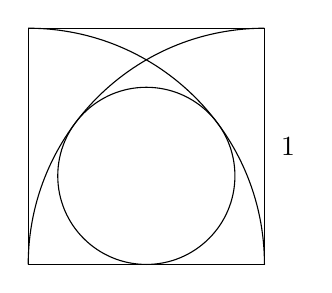
\begin{tikzpicture}[scale=3]
        \draw (0, 0) -- (0, 1) -- (1, 1) -- (1, 0) -- cycle;
        \draw (1, 0) arc[start angle=0, end angle=90, radius=1];
        \draw (1, 1) arc[start angle=90, end angle=180, radius=1];
        \node[label] at (1.1, 0.5) {1};
        \draw (0.5, 3/8) circle [radius=3/8];
    \end{tikzpicture}
    
    \item
    Siddharth and Dan are playing a tennis match. For each point there is a probability of $p$ that Siddharth wins. What is the probability that Siddharth wins the game?    
    
    \item
    A triangle $T$ has side lengths $a$, $b$, and $c$ where $c$ is the longest side length. Prove that: $T$ is right-angled $\iff$ $a^2 + b^2 = c^2$.
    
    \item
    \begin{enumerate}
        \item Evaluate $\int \limits_{-\pi}^{\pi} |\sin x + \cos x|\text{ }\mathrm{d}x$.
        \item Find $\int \sec x \text{ }\mathrm{d}x$ and $\int \mathrm{cosec} x \text{ }\mathrm{d}x$.
        \item Evaluate $\int \limits_{0}^{1} (1-\sqrt{x})^n \text{ }\mathrm{d}x$.
    \end{enumerate}
    
    \item
    You are walking along a route in a city with square blocks. You need to travel six blocks North and and six blocks East. The shortest possible route is therefore twelve blocks. How many different such twelve-block routes exist?
    
    \item
    Let $ABCD$ be a quadrilateral. Let $A'$ be the midpoint of $AB$, $B'$ the midpoint of $BC$, $C'$ the midpoint of $CD$, and $D'$ the midpoint of $AD$. Draw the lines $A'C'$ and $B'D'$, and let their point of intersection be point $M$. Let $a$ be the area of quadrilateral $D'MA'A$, $b$ the area of quadrilateral $A'MB'B$, $c$ the area of quadrilateral $B'MC'C$, and $d$ the area of quadrilateral $C'MD'D$. Prove that $a + c =  b + d$.
    
    \item
    Let $ABC$ be a triangle with $\angle CAB$ being a right angle. The point $L$ lies on side $BC$. A circle passing through points $A$, $B$, and $L$ meets the line $AC$ again at a point $M$ and the circle passing through points $A$, $C$, and $L$ meets the line $AB$ again at a point $N$. Prove that $L$, $M$, and $N$ are collinear.
    
    \item
    In Secret Santa, a group of people each pick out the name of a single other person at random, such that no one picks out their own name. In a Secret Santa group of $n$ people, find in terms of $n$ the probability that everyone picks out the same person that picked them.
            
    \item
    Jacob the gnome wizard is floating in space in the vicinity of a planet and no other bodies. As Jacob starts hurtling towards the planet, he decides to have one last adventure: to calculate the time until he dies on impact. What is the time in terms of the initial distance $r$, the initial velocity $u$, and the mass of the planet $M$, given that $u \leq \sqrt{\frac{2GM}{r}}$?
    
    \item
    Newton's law of cooling states that the rate of heat transfer of a body is directly proportional to the difference between the temperature of the body and that of its surroundings. This leads the objects to tend towards the same temperature. A can of Coke with temperature 15 degrees is placed in a fridge kept at constant temperature of 5 degrees. Given that it takes 2 minutes for the can of coke to reach 10 degrees how long does it take to reach a temperature of 7.5 degrees?
    
    \item
    $n$ points are placed on the circumference of a circle, and each pair of points is joined by a straight line. The points are chosen so that no three of these lines pass through the same point. In terms of $n$, how many regions is the circle's interior cut into?
    
    \item
    How many ways are there to select a list of $r$ objects from a list of $n$ possible options where each object can appear multiple times and order doesn't matter?

    
    
    
    
    
    
\end{enumerate}



\end{document}
